\documentclass[pdftex,11pt,a4paper]{article}
%\usepackage{parskip}
\usepackage[margin=1in]{geometry}
\usepackage{amsmath}
\usepackage{array}
\usepackage{caption}
\usepackage{hyperref}
\usepackage{subcaption}
\usepackage[pdftex]{graphicx}
\newcommand{\HRule}{\rule{\linewidth}{0.5mm}}
%\usepackage{parskip}
\renewcommand*{\sectionautorefname}{Section}
\renewcommand*{\subsectionautorefname}{Section}
\renewcommand*{\subsubsectionautorefname}{Section}

\begin{document}

\begin{titlepage}
    \begin{center}
        
\includegraphics[width=0.70\textwidth]{./assets/imperial.eps}~\\[1cm]
        \textsc{\LARGE Group Project} \\[0.5cm]
        \HRule \\[0.4cm]
        {\huge \bfseries Sight Reading for Cyborgs \\[0.4cm]}
        \HRule \\[1.5cm]
            \begin{flushleft}
                \large
                \emph{Authors:}\\
                Liam \textsc{Barden}\\
                Conrad \textsc{Godfrey}\\
                Guillaume \textsc{Lacroix}\\
                Megan \textsc{Lalla-Hamblin}\\
                William \textsc{de Renzy-Martin}\\
            \end{flushleft}
            \begin{flushright}
                \large
                \emph{Supervisor:}\\
                Dr William J. \textsc{Knottenbelt}
            \end{flushright}
        \vfill
        {\large \today}
    \end{center}
\end{titlepage}


\renewcommand{\abstractname}{Executive Summary}
\begin{abstract}
We have created Sight Reader, an application which reads and plays sheet music on your Android device. 
\\[1\baselineskip]
Optical music recognition has been researched since the 1960s and is still actively researched to this day. However, while almost all existing solutions interpret music captured using a desktop scanner, or from a PDF source, our application is portable and handles photos taken by a mobile device camera. This provides a number of interesting problems and challenges, for example image distortion and lower processing power on mobile devices.
\\[1\baselineskip]
Our solution allows a user to take a photo, or a series of photos, and output them as an industry standard MIDI file, which can be viewed and edited by a range of existing applications. This service would be invaluable for a novice musician trying to learn a challenging new piece, to play the second part of a duet with a soloist who finds themself without a musical companion, or simply to archive a piece of music for later use.
\end{abstract}

\tableofcontents
\listoffigures
\listoftables
\section{Introduction}
\subsection{Motivation}
Motivation!

\section{Background}
    \subsection{Musical Notation}
        In order properly to understand the task of reading music, one must understand a few basic terms.

        \subsubsection{Pitch}
            The pitch of a note is referred to by one of the first 7 letters of the alphabet, i.e. \{C,D,E,F,G,A,B\}.
            In scientific pitch notation, a number from 0 - 8 is added after the letter to indicate which octave the note is in.
            The lowest note possible in this notation, C0, represents a sound with frequency 16.35Hz, and the heighest possible, B8, has a frequency 7902.13Hz.
            A4 (frequency 440Hz) is considered an octave lower than A5 (frequency 880Hz), and an increase in octave represents a doubling of frequency in the sound produced.
        \subsubsection{Duration}
            In addition to pitch, notes also encode information about their duration, or how long the sound should be played. 
            Rests indicate an absence of sound. Both these durations are encoded as in Table \ref{table:notes}

            \begin{table}[h]
                \centering
                \begin{tabular}{| >{\centering\arraybackslash}m{1in} | >{\centering\arraybackslash}m{1in} | >{\centering\arraybackslash}m{1in} |}
                    \hline
                    Name & Note & Rest \\ \hline
                    Semibreve& 
                            
\includegraphics[width=20mm]{./assets/whole.png}
                            &
                            
\includegraphics[width=20mm]{./assets/wholerest.png} \\ \hline
                    Minim& 
                            
\includegraphics[width=20mm]{./assets/half.png}
                            &
                            
\includegraphics[width=20mm]{./assets/halfrest.png} \\ \hline
                    Quaver&
                            
\includegraphics[width=20mm]{./assets/4er.png}
                            &
                            
\includegraphics[width=20mm]{./assets/4errest.png} \\ \hline
                    Semiquaver&
                            
\includegraphics[width=20mm]{./assets/8th.png}
                            &
                            
\includegraphics[width=20mm]{./assets/8threst.png} \\ \hline
                    Crotchet&
                            
\includegraphics[width=20mm]{./assets/16th.png}
                            &
                            
\includegraphics[width=20mm]{./assets/16threst.png} \\ \hline
                \end{tabular}
                \caption{Note and Rest Durations}
                \label{table:notes}
            \end{table}
        \subsubsection{Stave}
            A stave comprises five horizontal lines and four spaces. A note can sit either in a space or on a line, and the height of the note dictates its pitch.
            \begin{figure}[ht!]
                \centering
                
\includegraphics[width=90mm]{./assets/staff.png}
                \caption{The Stave}
                \label{image:stave}
            \end{figure}
        \subsubsection{Clef}
            The pitch of a note on a stave is dependent on the Clef appearing at the start of said stave. There are two types, as below.  
            \begin{figure}[h!]
                \centering
                \begin{subfigure}{0.4\textwidth}
                    \centering
                    
\includegraphics[width=20mm]{./assets/trebleclef.png}
                    \caption{Treble Clef (or G Clef)}
                    \label{image:trebleclef}
                \end{subfigure}
                \begin{subfigure}{0.4\textwidth}
                    \centering
                    
\includegraphics[width=20mm]{./assets/bassclef.png}
                    \caption{Bass Clef (or F Clef)}
                    \label{image:bassclef}
                \end{subfigure}
                \caption{The Clefs}
                \label{image:clefs}
            \end{figure}
        \subsubsection{Bar}
            A bar is a division of time into a number of beats. Each bar is separated by a bar line.
            Separation of music into bars makes music easier to follow.
            \begin{figure}[h!]
                \centering
                
\includegraphics[width=20mm]{./assets/barline.png}
                \caption{Barline}
                \label{image:barline}
            \end{figure}
        \subsubsection{Time Signature}
            Time signature indicates the number of beats in each bar. A time of 4/4 (or C - common time) indicates there should be four crotchets (a.k.a. quarter notes) in each bar; 3/4 indicates there should be 3 crotchets; 2/4 - 2 crotchets; 2/2 - 2 minims etc.
            \begin{figure}[h!]
                \centering
                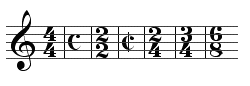
\includegraphics[width=70mm]{./assets/timesignatures.png}
                \caption{Common Time Signatures}
                \label{image:timesignatures}
            \end{figure}
        \subsubsection{Beams}
        Beams link together two or more consecutive quarter notes (or smaller divisions) to indicate a rythmic or melodic grouping, e.g. multiple notes for a single sung syllable. 
            \begin{figure}[h!]
                \centering
                
\includegraphics[width=20mm]{./assets/beam.png}
                \caption{Beamed Notes}
                \label{image:beam}
            \end{figure}
        \subsubsection{Dots}
            A dot after a note indicates that the note should be played for 1.5x normal duration, e.g. a dotted minim has the same duration value as a minim and a crotchet combined.
            \begin{figure}[h!]
                \centering
                
\includegraphics[width=20mm]{./assets/dotted.png}
                \caption{Dotted Note}
                \label{image:dotted}
            \end{figure}
        \subsubsection{Accidentals}
            Accidentals change the pitch of the note they are associated with. A sharp increases the pitch by a semitone (the difference between a B and a C). A flat decreases the pitch by a semitone. A natural accidental nullifies any changes to the pitch.
            \begin{figure}[h!]
                \centering
                \begin{subfigure}{0.3\textwidth}
                    \centering
                    
\includegraphics[width=20mm]{./assets/sharp.png}
                    \caption{Sharp}
                    \label{image:sharp}
                \end{subfigure}
                \begin{subfigure}{0.3\textwidth}
                    \centering
                    
\includegraphics[width=20mm]{./assets/flat.png}
                    \caption{Flat}
                    \label{image:flat}
                \end{subfigure}
                \begin{subfigure}{0.3\textwidth}
                    \centering
                    
\includegraphics[width=20mm]{./assets/natural.png}
                    \caption{Natural}
                    \label{image:natural}
                \end{subfigure}
                \caption{Accidentals}
                \label{image:accidentals}
            \end{figure}

    \subsection{Computer Vision and OMR}
        \subsubsection{OpenCV}
            OpenCV\cite{OpenCV} is an open source Computer Vision library. It is written in Native C++. We are using OpenCV4Android\cite{OpenCV4Android} which allows us to work completely in Java. This then calls the original C++ implementation through the Java Native Interface (JNI)\cite{JNI}. We have used the OpenCV library for two things: firstly to implement a camera, secondly to process the images.

        \subsubsection{Representing Images}

Bitmaps are perhaps the simplest method of representing an image. A bitmap is simply a 1 to 1 mapping for the value of each pixel in an image. Usually, bitmaps have multiple 'channels' to store multiple values for each pixel. The convention for digital photographs is to have 3 channels, one for Red, Blue, Green. This is known as the RGB format.

However, many existing computer vision techniques work only on a single grayscale channel, or even on a binary (black and white) image. Therefore, pre-processing is sometimes required.

In this project we have used the Android implementation of Bitmaps\cite{Bitmap}.

        \subsubsection{Grayscale Conversion} \label{sec:grayscale}

Converting a full color image to grayscale is a relatively simple operation. For each pixel in the image, you simply find the average value of each color channel. The new image can be represented by a single channel, which reduces the memory requirements 3-fold. Obviously, some information will be lost in this process as many different colors will map to the same grayscale value. However, sheet music does not assign any semantic meaning to different colors and so this is not an issue for our project.

        \subsubsection{Image Thresholding} \label{sec:threshold}

Converting a grayscale image to a binary (black and white) image is also a simple process. A threshold is chosen and all intensity values below the threshold are set to black while all values above it are set to white. The \lq intensity\rq of a grasycale pixel simple refers to that pixels value from 0-255. However, deciding on this threshold value is a non-trivial problem and is explored further in our implementation.   
\[ f(i,t) = \left\{ 
  \begin{array}{l l}
    255 & \quad \text{if } i \leq  t\\
    0   & \quad \text{otherwise}
  \end{array} \right.\]

        \subsubsection{Erosion and Dilation} \label{sec:erosion}

When you want to detect a specific feature of an image it can often help to emphasise that feature through image processing. Erosion and dilation are two common ways in which this might be done.

Eroding an image means to expand the black areas of the image, while dilating means to expand the white areas of the image. This has a wide variety of applications such as removing noise, filling small gaps and highlighting important features.
            \begin{figure}[ht!]
                \centering
                
\includegraphics[width=90mm]{./assets/dilated.png}
                \caption{Erosion/Dilation}
                \label{image:dilationerosion}
            \end{figure}

For processing the algorithm that does this requires a kernel and iteratively goes through each pixel in the image. For each of them it runs the convolution with the specified kernel, making calculations depending on the surrounding pixels intensity as well as the kernel values, and returns a value that will state whether the given pixel becomes black or white. Intuitively, this kernel can be thought of as a matrix represents the area around each pixel to look into, centred on the pixel of interest. A change in the shape or size of the kernel can lead to totally different processing effects. The effect will also depend on the quality of the image and the lighting conditions.

It is important to note that each eroding/dilating operation requires some thinking and testing about its kernel shape and size.

\subsubsection{Projections} \label{sec:projections}

There are two basic types of projections: horizontal and vertical. A horizontal projection performs an operation on each row of the image. You end up with a new image of width 1 and the same height as the original image. In our case, we always average the values in the grayscale image channel.
Similarly, a vertical projection performs the same operation on columns and outputs a new image of height 1 and the same width as the original image. The operation we use is also the average of the intensity values.

\begin{figure}[h!]
	\centering
	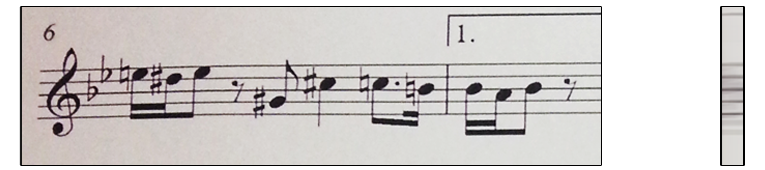
\includegraphics[width=1\textwidth]{./assets/projectionBackground.png}
	\caption{An example image with its corresponding horizontal projection}
	\label{image:projectionBackground}
\end{figure}

\subsubsection{Contours} \label{sec:contour}

A contour is a boundary between two areas of different color in an image. On a black and white image, this will separate the black from the white areas. The built-in method \verb!findContours!\cite{findContours} in the OpenCV library finds all contours in a given image, returned as a list of matrices, by following a complex algorithm that is outside the scope of this document. The contour can then be processed to find useful information such as its center of gravity.

Intuitively, the center of gravity of a shape represents the point that a human would call its 'center'. For a highly symmetric shape, like a circle or star, this will be located in the geometric center of the shape. For an uneven shape, like a hammer, the center of gravity may be quite far from the geometric center of that shape.

We can find the center of gravity of a contour using the following formulae:
\begin{equation}
    x = \frac{ m_{1,0}}{m_{0,0}}
\end{equation}
\begin{equation}
    y = \frac{m_{0,1}}{m_{0,0}}
\end{equation}
where $m_{i,j}$ denotes the $i$th moment on $x$ and $j$th on $y$



\subsubsection{Hough Transforms} \label{sec:hough}

Hough transformations are feature-extraction techniques that work by transforming the image into a new mathematical space where the desired feature is highlighted. The two most commonly used Hough transformations are Hough lines and Hough circles, which detect straight line segments and circles respectively.

The Hough lines transformation highlights the location, direction and length of all lines on that image. Points above a given threshold are then extracted from this image and converted into line segments.

It can be very useful for detecting long, thick lines in a source image but it does not perform well with short or thin lines. Also, because the algorithm is probabilistic, small lines that are next to a larger line may be considered noise and be ignored. Also, if a line is even slightly bent then it will register as several smaller lines or possibly not be detected at all. Finally, the algorithm is very slow as it checks every pixel in the
image, which is a serious problem for an Android device as it has little processing power.

Hough circles is a similar algorithm that detects circles in an image. It has similar strengths and weaknesses to Hough lines.

\subsubsection{Template Matching} \label{sec:template}

Template matching is a technique for detecting complex, arbitrary patterns in a source image. It searches the source image for areas that best match a given 'template' image.

It works by performing the following check on each pixel of the source image. Starting from that pixel, we select an area of the source image of equal size to our template. Then, we can check how well that area matches the template by comparing each pixel to its corresponding pixel on the template and then combining these results. 

Once we have done this for each pixel in our source image, we can extract all the matches that are above a certain threshold. While doing this, we must consider that if one pixel is a good match, the pixels surrounding it are likely to be good matches too and so we require a minimum distance between any 2 matches.
    
            \begin{figure}[h!]
                \centering
                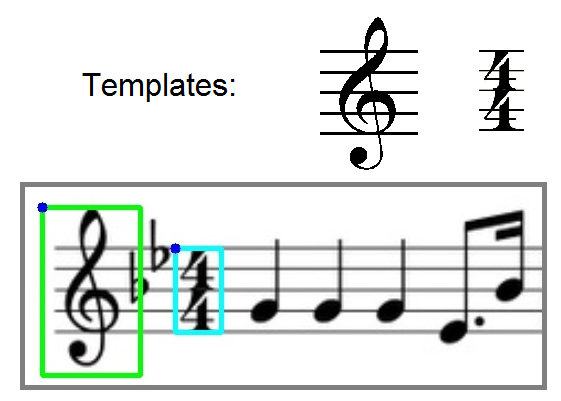
\includegraphics[width=90mm]{./assets/templatematch.png}
                \caption{Best matches for 2 different templates}
                \label{image:templatematch}
            \end{figure}

Another important consideration is the selection of a pixel comparison method. It is perhaps counter-intuitive, but it is not enough to simply check which method gives the best matches. Rather, we need to find the method that gives the most distinct results, ie. the greatest difference between the least accurate positive match and the most accurate negative match. This is because the method uses a threshold value to determine
which values constitute a match, and this threshold must fit within our tolerance gap.

As expected from looking through the literature, we found that the 'correlation-coefficient' approach gave us the best results and we used it throughout the project.  
It is given by the following equation:
\begin{equation}
	C(x,y) = \sum_{x'y'} T'(x',y') I(x+x',y+y')
\end{equation}

where $x'$, $y'$ sum over the dimensions of the template image, and $T(x,y)$ and $I(x,y)$ return the intensity values found at those coordinates in the template and source image respectively.
The major advantage of template matching is its ability to match an arbitrary pattern. While most other algorithms are highly specialised to detect a single feature like straight lines, template matching can find virtually any distinctive pattern in an image. However, this also presents its greatest drawback: it searches for a very specific pattern and is therefore very intolerant to slight variations in this pattern. It
is also slow as it operates on each pixel in the image.

Another drawback of template matching is that there is no built-in method to extract more than one result. While there exists a method, \verb!minMaxLoc! in the org.opencv.Core package, that returns the location and value of the best result there is no trivial way to extract any further results. The way we worked around it was by zeroing all the pixels in a specified area around the best result and calling \verb!minMaxLoc! again until the associated value reached a certain threshold. This threshold has to be fine tuned for each feature we want to template match.

For best results the technique should be used on a very specific and distinctive pattern. It should typically be used when more specialised solutions are not applicable.

    \subsection{Android}
When working with Android the provided paradigm for managing the flow of your application is through the use of Activities. As described in the android developer guide:

\begin{quote} 'An activity is a single, focused thing that the user can do. Almost all activities interact with the user, so the Activity class takes care of creating a window for you in which you can place your UI' - \href{http://developer.android.com/reference/android/app/Activity.html}{Android Reference}
\end{quote}  

The app starts with a main activity which can then cause other activities to be started to do different tasks. Activities are kept on the 'back stack', which operates on the normal first in last out (FILO) order. When a new activity is started it gets added to this 'back stack', when that activity finishes we go back to the activity before, similarly when the device back button is pressed. This means that by using
activities in our app it enables the user to move through the app as they are used to using the back button as usual. Also if the app is minimised and then reopened it will retain its place.


\section{Design and Implementation}

\subsection{Platforms and Language Choice}

Since this application is built for Android tablets, we had to either write our application natively in Java with the Android SDK, or use a middleware platform. We ultimately chose the native approach due to several considerations. We needed to access external sdk’s and libraries that may not have been supported by any given middleware platform. We also did not require the major benefit of using such a platform (cross-platform compatibility, eg. with iOS) and also many of the better ones are neither open source nor free. 
Once we had decided to go with native java, we had to choose a computer vision library. The obvious choice was to go with OpenCV as it is widely used, open source, powerful and has a variety of useful features. We also ended up using a library called FileDialog (CIT) for our file dialogs, and Android MIDI library to generate our MIDIs.

\subsection{Application Layout}

Once the language and libraries were chosen, we decided to start the design of the application. This original design has only suffered from minor changes until the end. There are 3 main parts: 
\begin{enumerate}
\item{The Android application}
\item{Music detection}
\item{Interpreting and playing back the music}
\end{enumerate}

(IMAGE)


\subsection{The Android Application}

            \begin{figure}[ht!]
                \centering
                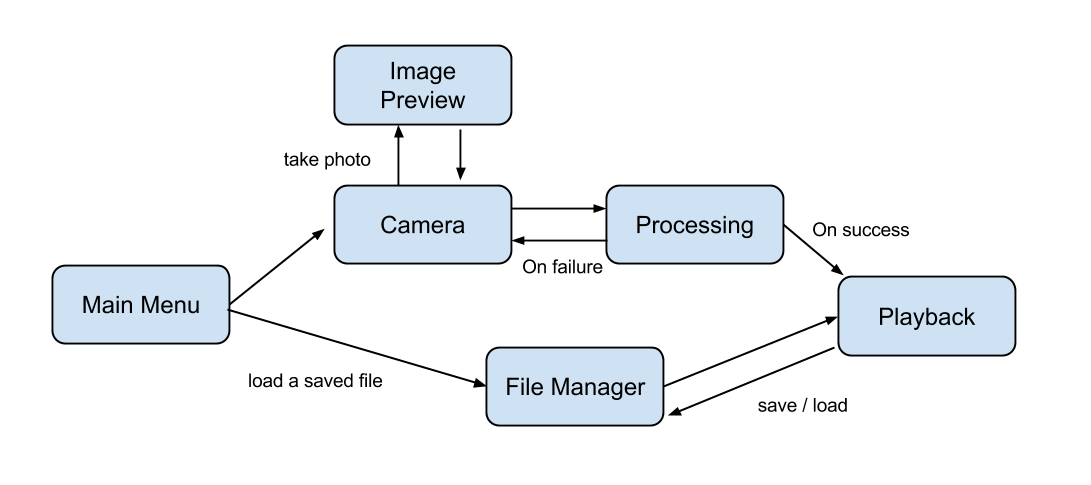
\includegraphics[width=150mm]{./assets/activitiesdiag.png}
                \caption{A flowchart of activities in the application}
                \label{image:activitydiag}
            \end{figure}

\subsubsection{Activity Layout}

The main activity for the app is SightReaderActivity. The app home screen has two options, Scan and Play.

[home screen capture] [Scan screen capture]

The Scan option launches the CameraActivity which takes you to the capture part of the app where you can take a picture of some sheet music. Tap the camera preview to take a picture, this launches the DisplayPhotoActivity which allows you to decide if you want to keep the picture or try again. You are then returned to the Camera preview screen. Once you have captured as many pictures as you want you tap done and the ProcessingActivity is called and the processing begin. Here we have a
processing screen as this can take some time to let the user know the app is still running.

[displayphotoactivity capture][progress screen capture]

The reason for using a new activity for each new action is that this allows each activity to handle normal function such as when the back button is pressed in the intuitive way. This is the recommended method of organising android apps as discussed in the background section.

The other option is to press ‘Play’ which takes you to the file management dialog. Here, you can view the midi files all of your previously processed pieces. Selecting a saved piece will then take you to the playback activity where you can hear it. We have used the FileDialog library, detailed in the background section, to implement this functionality. We have configured configured to open in the default save file directory with a filter to only show the relevant files.

[screen capture??]

\subsubsection{Camera Considerations}
We originally used the default android camera activity for taking the photographs, but later realised that we required additional features that this activity could not handle. Therefore, we implemented a new camera activity called SightReaderCameraView so that we could keep the theme of our app consistent and also have finer grained control on the camera options to maximise our detection accuracy.

\subsubsection{Saving Files}
\[Diagram here\] 
We need to save various files, both so the user can reaccess past music and also in order to deal with the limitations of device RAM.

\subsection{Music Detection}

Understanding sheet music is quite a complicated problem. The semantic meaning of the music is highly dependant on the relative locations of various features on the sheet. Understanding an English sentence is very simple, by contrast. Each letter is read sequentially from left to right, lines from top to bottom, and the spaces between letters denote words. When it comes to musical notation, however, even very small variations in the location of elements can entirely change the sound it
transcribes. This provides us with a significant challenge: we need precise and accurate detection methods if we want reliable results.

\subsubsection{Our Solution}

Broadly speaking the algorithm we created works as follows: 

\begin{enumerate}
\item{The photograph is taken and the images are rescaled and prepared for detection.}
\item{We pull out the staves from the image. They tell us where to look for the other features.}
\item{We sequentially extract each musical feature from the image, such as notes, clefs etc. Each pass can build on previous knowledge, eg. the beams between notes can take advantage of knowing the note locations.}
\item{We then use the relative locations of these features to determine the semantics of the musical piece.}
\end{enumerate}

Since there is no general way to detect an arbitrary feature using OpenCV, we had to try a wide variety of different methods based on our - admittedly small - prior knowledge of computer vision, what we learnt during first term, what we could find in different papers related to this question and what we could find in OpenCV tutorials. A detailed summary of the implementation of each step is explained below.


\subsubsection{Implementation Details}

\paragraph{Pre-processing}

As sheet music does not assign semantic meaning to colors, we decided to first remove all color from the image using a grayscale conversion. We then thresholded the image to increase image consistency in different lighting conditions. These processes are detailed in the background section.

Secondly, the convention in computer vision is to use white-on-black images. However, sheet music is the opposite, black markings on a white page. This means that before we do anything, we need to invert the image. This can be done very quickly by bitwise operations, ie. applying bitwise NOT to each pixel.

When we later transitioned from scanned pdf images onto real photographs we discovered a significant flaw with our preprocessing algorithm. On a photograph you are very likely to have shadows (including the shadow of the device taking the picture) and this means that some areas of the image are darker than others and therefore require a different threshold. We even found that on many images there did not even exist a single threshold value that could describe the entire
image. Therefore, we needed a method of finding the correct threshold dynamically.

(IMAGE) 

We solved this by first dividing the image into small, equal sized sections and found the average color of each section. As the image is going to be mostly black (a music sheet is mostly white space, and we have inverted the image) this means that features will be significantly lighter than this average. We therefore increase the average by a fixed percentage and use that as our threshold for that given section. Then, the sections are recombined back into a final binary image. We are now
ready to begin detecting features.

\paragraph{Staves}

The staves are perhaps the single most important feature when it comes to detection.  All of the other elements on the page gain semantic meaning based on how they are placed relative to a stave. For example, notes determine their pitch based on their Y location on the stave lines. Therefore, we needed an accurate and robust detection method. We broke the problem into 2 halves, detecting all of the lines and then building the staves out of that pool of lines.

\subparagraph{Detecting the lines}

Our first attempt to recognise the lines was to use the standard ‘Hough Lines’ algorithm. However, this approach had very serious problems with detecting the thin stave lines accurately, as explained in the background section.

After this obvious approach had failed, we decided to look into the literature and found that most previous work used a horizontal image projection to solve this particular problem (CIT). By horizontally projecting the image onto a single column of pixels, we could detect large horizontal lines on the page and from there extract the stave information. (IMAGE)

This proved simple to implement using OpenCV and served us very well for some time. We did not realise the fatal drawback to this approach until we moved from pdf images to images taken with a smartphone camera. 

\subparagraph{Correcting Line Distortion}

On computer generated pdf images, the stave lines are always exactly horizontal and evenly spaced. This is how the horizontal projection can reliably extract the lines from all the surrounding noise. However, on a photograph this is an entirely unrealistic assumption. We identified 4 separate types of image distortion that undermine this algorithm’s effectiveness.

\begin{enumerate}
\item{Angular distortion when the camera is not perfectly aligned with the axes of the image.}
\item{Lens distortion from the camera causes slight bulging as you move towards the edge.}
\item{The paper may be slightly crumpled leading to sudden changes in line direction.}
\item{Perspective may lead to different lines having different degrees of distortion.}
\end{enumerate}

As all of the previous research has focused on scanned or generated images, we could not find a solution for distorted stave lines in the literature. We ultimately arrived at a novel solution (to our knowledge) for solving the issue, outlined as follows.

We first break the image down into several equal-sized vertical strips, similar to how a paper shredder works. The thinner a strip is, the lower the distortion is relative to the length of the line, and so below a certain width even moderately large distortion becomes negligible. We found that 30 strips offered a good compromise between accuracy and speed. Then, each of these thin strips have a horizontal projection performed on them. The line segments are
then extracted from these projections and are ‘threaded’ back together, by connecting lines on adjacent strips that are within a certain Y distance. Once the lines have been reconstructed, all viable lines (which are long enough to qualify) are saved. (IMAGE)

\subparagraph{Building Staves from Lines}

The second half of the problem turned out to be much simpler. We had to take this pool of lines and extract staves, ie. groups of 5 lines with even spacing and width. This was done by sorting the lines vertically and then selecting each and every pair of lines. The pair was assumed to be the first 2 lines of the stave, and then the algorithm would check for 3 more lines with the same spacing below that pair. If all 5 lines are detected, the lines
are removed from the pool and saved as a stave.

An additional problem we found was that on pages with 5 or more staves, the algorithm could incorrectly detect a set of 5 equally spaced lines from different staves. For example, the first line of each of the 5 staves might be recognised as a stave itself. We solved this trivially by specifying a maximum spacing between stave lines. (IMAGE)


A final issue we ran into much later was that in cases where the image was at least moderately distorted, a single straight line could not accurately describe the location of a stave line on the paper, and so we had to keep the reconstructed lines from the detection algorithm rather than simply using their best-fit approximation. (IMAGE)

Now that we have a reliable method for detecting the staves, we can use this information greatly speed up the detection of other elements, by only looking in specific locations for them.  For example we know that a clef will only occur at the far left of a stave and so we only need to search a very small area of the page. It also allows us to give semantic meaning to many other musical features, such as determining the pitch of notes.

\paragraph{Clef and time signature detection}

Despite their unique shape, clefs and time signatures do not have any particular characteristics that are easily exploitable to differentiate them, regardless of any eroding/dilating we may run first. This forced us to use a template matching algorithm to detect them. The way this is done is that we store an image for each feature that we want to detect - treble clef, bass clef, 4/4, 3/4, 2/4, 3/8, 6/8 time signatures, and run a separate
template match on each of these.

\subparagraph{Extracting the results}

Although there is a clef at the beginning of each stave, and a time signature at the start of each music piece, there is a need to run the detection on the whole piece because additional clefs and signatures can be found at an arbitrary point in the staves.

The matrix ‘returned’ by ‘matchTemplate’ is of size:

\verb!(imageHeight - templateHeight + 1, imageWidth - templateWidth + 1)! .

Each cell of the matrix is an area of size one storing a double corresponding to the value computed in regards of the comparison method used at the given pixel location in the image. Since they are stored in arrays, results are difficult to extract directly using an intuitive algorithm. Fortunately,there exists a built-in method of OpenCV, ‘minMaxLoc’, which returns an object storing the maximum and minimum value in the matrix of this type, as well as their respective locations - both are stored because depending on the comparison method used, the best results will be stored either at the maximum value location, or the minimum one.

With this method, we can extract a value that is then compared to a threshold, either calculated at the start of the method, or being set in terms of percentage of the first (therefore best) match, or a constant one if the comparison method is used in its normed way. If this value passes the threshold test, the associated location is a good match. The location is then added to the corresponding list (e.g. treble clefs list if we’re running the treble clef detection).

/* Proofreading needed for the next paragraph, not sure it actually means anything in English */

So far we have found the best match in the image. Unfortunately, the ‘minMaxLoc’ method does not remove the values from the matrix. We then have to set the values in the matrix to zero, at the just-found location but also around it to prevent another match just next to the previously found location, that would correspond to the same feature: we set all values in the areas around the point, in all directions and for the
size of the template image to zero, and iteratively run the extraction algorithm again until the threshold test fails. We have then found all features for the given method.



            \begin{figure}[ht!]
                \centering
                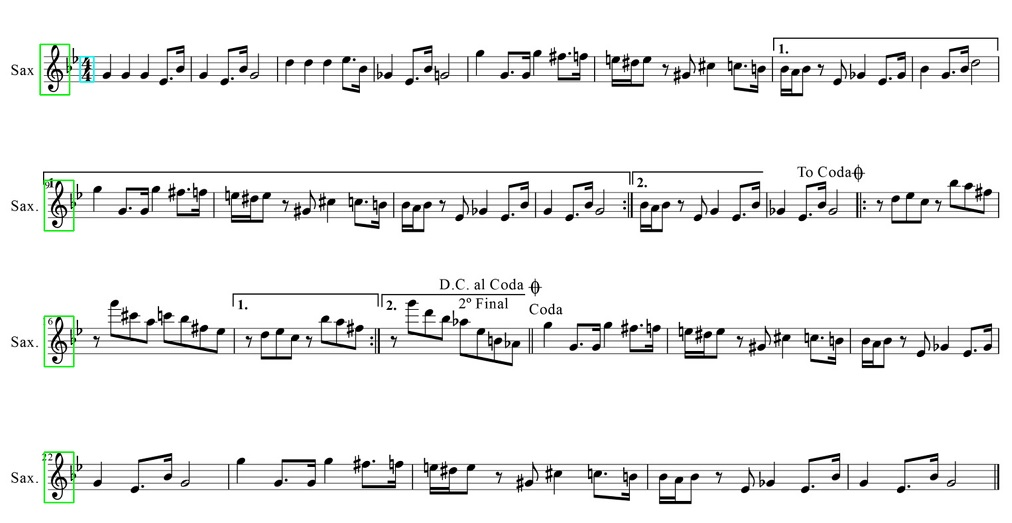
\includegraphics[width=1\textwidth]{./assets/detectedfeatures.jpg}
                \caption{All detected features through clefs and time signatures detection}
                \label{image:detectedfeatures}
            \end{figure}


Due to the uniqueness of their shapes, this gives excellent results in accuracy, with only 10\% of difference in the values between the best positive match and the worst positive match, and 45\% between the best positive match the best negative match. Unfortunately, it is also very time consuming with images this large, which is the reason we try to avoid using template matching as much as possible in the different
methods of detection.

\paragraph{Crotchets}

There are many ways to detect crotchets. Unfortunately, most of them do not only recognise crotchets but also accidentals, beams, lyrics or sometimes just noise. We had to try many methods before finding a reliable one.

\subparagraph{Hough Circles}

We originally tried to make use of the ‘Hough Circle’ algorithm. The method ‘HoughCircles’ is provided with OpenCV is very easy to use and merely depends on any variable: only the minimum distance between two detected circle centers is to be changed, as well as the minimum/maximum radius of the circles to detect. It was therefore quite straightforward to test the method. However, even when combined
with highlighting techniques like eroding/dilating, this did not give any consistent results. There was a high rate of both false positives and false negatives. Considering the processing time that it took to run HoughCircles, we decided not to go further in this direction and changed the algorithm.

\subparagraph{Template matching}

Our first attempt was to use template matching. However, we quickly ran into a variety of non-trivial problems. Firstly, notes can have a tail either above or below its head, which would require us to use multiple templates. Additionally, the tails may not always be exactly vertical due to image distortion, which means we would either have to include even more templates, or risk sacrificing
detection quality by only matching against heads. Also, many features of sheet music look similar to note heads, as they are just a circular blob. This gave us a large nmber of false positives. Finally, different music notation programs use slightly different images for note heads, which would mean we need more templates still. Clearly, we needed a different approach.

\subparagraph{FindContours}

We settled on the following algorithm: after a very careful and measured eroding, we used the built-in 'findContours' method to detect all contours. Because the 'findContours' method is very accurate, we need to have a measured eroding that would get rid of all the noise without erasing any of the notes. Fortunately, since notes are almost round and compact, we can afford a very large
eroding kernel, resulting in loads of features being simply erased, as well as all noise.
Once a contour has been found, we used moments to recover the center out of them, as explained in the background. This approach can very quickly and accurately detect every single note on the page, with almost no false positives. It is also highly insensitive to noise because of the large erosion kernel.
\begin{figure}[ht!]
    \centering
    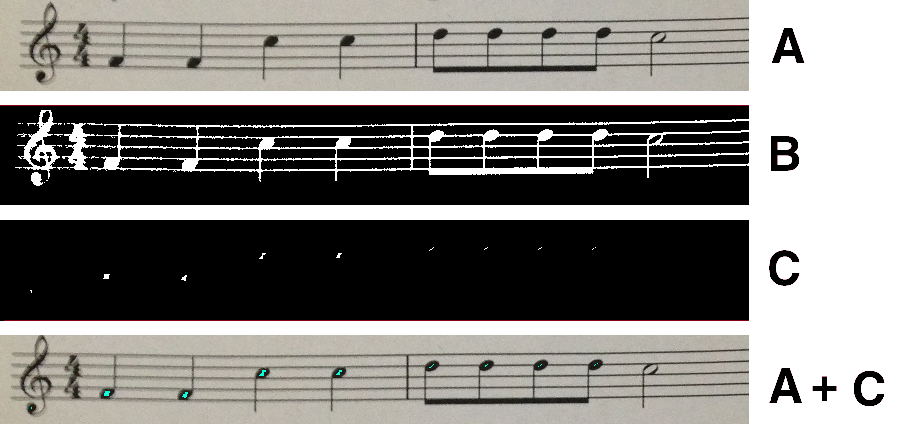
\includegraphics[width=1\textwidth]{./assets/highlight.png}
    \caption{Highlight of the computation of erosion for the purpose of crotchets detection}
    \label{image:highlight}
\end{figure}

We encountered some issues where beams would be mistaken for notes after the eroding, depending on the beam’s direction, slope, location and thickness.. Since it was sometimes very easy to mistake an eroded beam for a note, we also ran the same algorithm with a much lower erosion, leaving most of the beams intact. This allowed us to differentiate them from real notes,
catching the false positives. Notes are only recorded if they register as a note on both levels of erosion.

\begin{figure}[ht!]
    \centering
    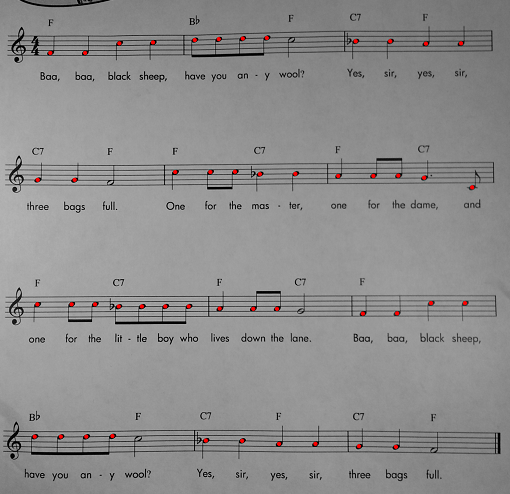
\includegraphics[width=1\textwidth]{./assets/crotchetsdetected.png}
    \caption{All detected crotchets are accurately detected through this algorithm}
    \label{image:crotchetsdetected}
\end{figure}

The notes are then ordered by x coordinate, which aids the detection of some of the following features.

\paragraph{Accidentals}

Similarly to clefs, the uncharacterised shapes of accidentals forces the use of template matching. But as opposed to clefs, we need not run the detection on the whole stave: we just run it on areas around the note, not too specific because of noise, small location errors and the actual position before the note which is not fixed, depending on the actual
position of the note and that of the neighbouring notes. Therefore, we run the template matching method on a fixed small area in front of each note.

\paragraph{Beams}

At first glance, beam detection may appear similar to stave detection. However, they are not necessarily horizontal which makes a horizontal projection impractical. Fortunately we can exploit the fact that they are very thick instead (compared to all other lines in sheet music).

First, we eroded the image to get rid of the small noise and stave lines which may interfere with detecting beams. We then used Hough lines to try and detect the remaining lines, naming only the beam lines. Unfortunately, we ran into the problem where Hough lines cannot detect lines of significantly differing sizes, as explained in the background. Due to the
significant processing overhead it introduced, we decided to find another approach.

First, we applied a strong erosion to the image. This left us with only the most prominent features, namely the notes and beams. Then, using our prior knowledge of the location of notes, we black out all notes on the eroded image, leaving us with just beams.

From here, we apply a vertical projection to the image, which picks out the x-dimension ranges of beams. Now that we know the x locations, for each x range we extract its vertical strip from the eroded image and we then perform a horizontal projection to also find their y locations.

There is an additional problem to consider, double beams are a common feature in sheet music and we wanted to support their detection. However, some of these double beams may be quite small as shown in \ref{image:beamsdetected} 


We solved this by taking the eroded image, after the first pass of the algorithm, and blacking out all the beams we detected in that pass. Then the detection can be run again to find the second beam in a double beam. This can be repeated again for triple beams and so on.


\begin{figure}[h!]
    \centering
    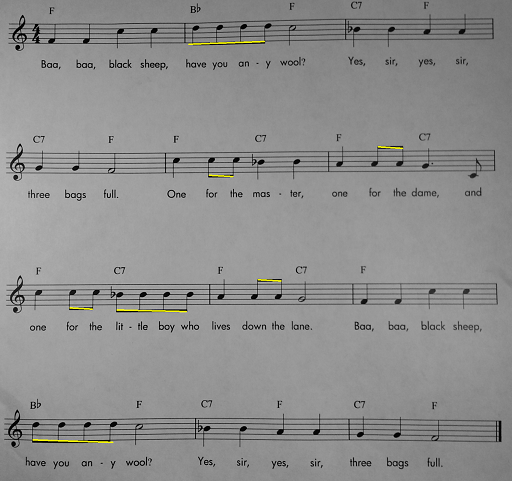
\includegraphics[width=1\textwidth]{./assets/beamsdetected.png}
    \caption{All detected beams after running the method}
    \label{image:beamsdetected}
\end{figure}

\paragraph{Quavers}

We do not check for quavers directly, rather we perform an extra check on each crochet to determine if it is next to a quaver tail. This is a 2-part process: first, we erode the image with a non-square kernel of width 2. This will erase the stave lines but keep the details of every feature with width greater than 2 pixels; which includes
quavers. We then isolate a small area to the right of the note and use the ‘findContours’ algorithm on this area. If a contour is detected that is tall enough to be considered a quaver tail rather than noise, we record that the note is a quaver.

\paragraph{Dots}

The only robust way to accurately detect dots is to use the findContours on some area after note, after some eroding, and check for the location of the center of gravity of the contours if it isn’t too wide or high, the same way we did for crotchets. This value is then compared to the expected location: the exact middle of
the stavelines. The difference in height is computed, using the accurate exact value of the stave positions at the given location. If it is small enough, the contour is validated as a dot, and the duration of the note is updated.

Contours are well suited to this problem as dots necessarily have a border of white space around them - otherwise they would not be a dot.

\begin{figure}[ht!]
    \centering
    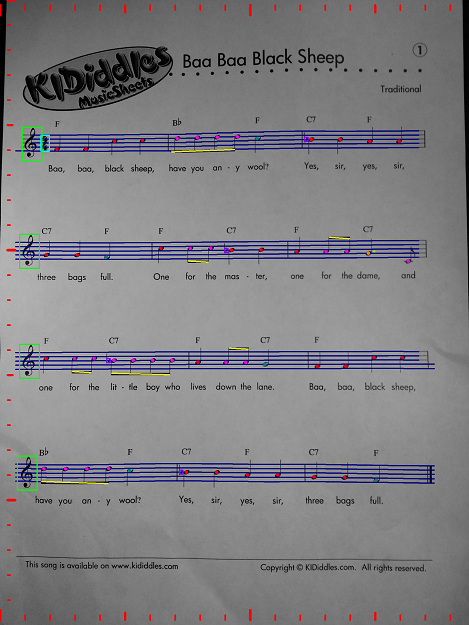
\includegraphics[width=1\textwidth]{./assets/detected.png}
    \caption{All detected features after running the whole application. For debugging purposes, a scale is printed as well. Each note color corresponds to a different duration of the note.}
    \label{image:detected}
\end{figure}

\subsection{Interpretation and Playback}
\subsubsection{Intermediary representation}
Once the music has been detected, we build up an intermediary representation of the piece. The structure of this representation is as follows:
The \verb!Piece! class holds information such as the clef, tempo and time signature of the piece. \verb!Piece!s contain a list of \verb!Bar!s, which themselves are lists of \verb!Chord!s, and a \verb!Chord! is a list of \verb!AbstractNote!s. There are then two subclasses of \verb!AbstractNote! - \verb!PlayedNote! and \verb!RestNote!. Notes contained information about their pitch, duration and velocity. We felt this intermediary representation was adequate for our immediate needs, but it was also open to any potential extensions we may desire later on.

\subsubsection{Playback}
Playback was achieved in two steps. First we generated a MIDI file from our intermediary representation. This was a case of iterating through the nested lists using the helper functions provided by the Android MIDI Library. This library provided an interface to the MIDI format through the class \verb!MidiFile!, which represented a series of \verb!MidiTrack!s. Tracks were manipulated by inserting events, and
a function \verb!MidiTrack.insertNote()! meant inserting either a rest or played note was straightforward. Once generated it was saved to the device. It can then be retrieved from the file system and played back using the Android JetPlayer Class.


\section{Evaluation}
    
    \subsection{Performance}
    We can breakdown the performance of our app into three major areas
        \begin{enumerate}
        \item{How accurately the detected music reflects the actual music}
        \item{The speed with which our app parses the sheet music}
        \item{The responsiveness and general flow of our app}
        \end{enumerate}
        \subsubsection{Accuracy of Detection}
            We tested the accuracy of the music detection by parsing various different test images and checking by hand how many of the features were correctly detected. We considered trying to automate this process when we first started the project, however we quickly realised that solving this automation problem would take just as much if not more time than solving the task itself. As such it is a method that has stuck with us since the beginning.
            The results of our most recent tests are seen in Table \ref{table:testresults}
            \begin{table}[h!]
                \centering
                \begin{tabular}{ c | c | c }
                    Piece Name & Distinct Feature Types & Percentage of Features Correctly Detected \\
                    Baa Baa Black Sheep & 8 & 100\% \\
                    Indiana Jones & 10 & 90\%\\
                \end{tabular}
                \caption{Test Results}
                \label{table:testresults}
            \end{table}
            
            All of the basic feature types, which is to say all the distinct feature types in "Baa Baa Black Sheep" are reliably detected in any piece we try to parse. However the more complex elements, such as the Rests in Indiana Jones are what cause problems for our detection system.
        \subsubsection{Speed of Detection}

        \subsubsection{Responsiveness}
    \subsection{Tool Choice}

    \subsection{Difficulties Encountered}

    
Our tests involved running the app on various different test images. We wanted it to do this fairly quickly/efficiently so we get a quick response for the user, which is important for apps. This led us to use a new algorithm because the old one was too slow.

We started by re-uploading all of our testing images every time we ran a test. This was a significant pain point in our project as each upload took in the region of 20-30 seconds, and when we had done it enough times so as to want to shoot somebody we decided to look at how we could refactor our code.

The device we are used primarily for development was the Motorola Xoom from 2011 running Android 4.2.2 with a 5MP camera. This meant we were working with a device which is not brand new and so the technology will be guaranteed to supported on older devices. The aim of this being that the app should work for a larger range of people than if we were using a newer device which might cause compatibility issues, or behave unacceptably slowly on slightly older devices. We have also
been using our android phones for testing which checks if they work on another device and also on a smaller screen.

Because of the visual nature of our task our testing techniques for the majority of the project had needed to be quite laborious, and relied on us looking over the outputs of our app to see that we were detecting the right pieces of musical notation when we were supposed to be, and not detecting things we were not supposed to be. For example, once we were able to detect the staves in our images reliably, we would then try and recognise the note heads in the images, and did not design
another element until we were able to “pass” the visual “test”. We did consider trying to automate a process like this, but we quickly realised that setting up that automation would be a task akin to completing our actual task, and so was not worth the time it would save.


In the app activity:
detector.print(output);


In MusicDetector.java:
public void print(Mat sheet) {
printStaves(sheet);
printFourFour(sheet);
printTreble(sheet);
printNotes(sheet);
printBars(sheet);
printFlats(sheet);
}


private void printNotes(Mat sheet) {
for (Note n : notes)
Core.circle(sheet, n.center(), (int) (staveGap / 2),
(n.duration() == 1. ? new Scalar(0, 0, 255)
: (n.duration() == 2. ? new Scalar(128, 128, 0)
: new Scalar(255, 0, 255))), -1);
}


We used print methods to check what has been detected visually.


If this was a larger scale project that did not have as a tight a deadline as the one we are working towards, we would have considered a more sophisticated testing strategy that automatically generated new sheet music from our intermediate data structure, and then tested the generated sheet music to see if it
matched up, but the task of generating sheet music from our data structure was deemed too time intensive.

Tools
We have been using gradle to build our project, some of the output of this is seen from Jenkins below, and our build.gradle content is posted below. We chose this build tool for two reasons: first of all, gradle is the basis of the official new build system for Android, which uses a DSL (Groovy) to write build
files and Groovy is very easy to work with coming from a Java background - which all of us in the team have. The second reason is that it manages dependencies using maven, and has the gradle wrapper, making it very easy for anyone to compile the project from scratch from anywhere (assuming they have the
Android SDK installed). As mentioned before, when Jenkins pulls from our GitHub repository it runs the gradle wrapper to compile the app. 


\section{Conclusion and Extensions}

When we started this project, we deludedly thought that 8 weeks in we would be able to scan Fantasie Impromptu by Chopin, one of the most musically complex and technically challenging pieces we could think of. While our goals may have shrunk, our pride in what we achieved hasn't. We have created an app that has laid the groundworks for a robust OMR system, and proven that it is possible to have decent music recognition on a mobile platform. 

As a team that were not only novices in computer vision, but also in the field of OMR, we had no idea what we could accomplish at the beginning of the project, so we decided to aim high, and then bring our expectations down as we progressed. We did not manage to accomplish all of our original goals; along the way we made the decision to prioritise finishing certain areas at the expense of others. This means that for example while we did not manage to support multiple staves or musical chords, we can say that our fundamental features of note detection and stave detection will work very reliably.
 
To improve the usability of the software, we could be able to display the interpreted music from within the app, as well as outputting it to MIDI which we already do. This could be used to feed a visual representation of the music back to the user, or be further manipulated from within the app. We could also allow users to select different musical instruments to play back the piece in, or give them the ability to change the tempo to aid in practice. To speed up the processing time, we could parallelise more operations to exploit the multiple cores found in modern mobile devices, or if the user is connected to the internet, send the job to a server with high processing capability.
 
To make the software more useful, we could add automated transposition of Music- a goal we mentioned early on in the report, we could add support for multiple stave recognition, and handling chords (multiple notes simultaneously). Both were left out due to time constraints, as we wanted to make what we did have quite robust rather than having an app with more features that didn't work 30\% of the time.

Also to make the app more marketable we would package OpenCV so that it can stand alone. As specified \href{http://docs.opencv.org/doc/tutorials/introduction/android_binary_package/dev_with_OCV_on_Android.html}{here}.
At the moment we are making use of OpenCV Manager which automatically downloads the best version of OpenCV for the development device.



\section{Project Management}
\subsection{Supervisorial input}
We arranged to have weekly meetings with our supervisor William Knottenbelt to keep him updated on the progress of our project, whilst also ensuring we felt we had a target to work to. We had an aggressive implementation schedule at the beginning of the project, and  This worked well for the first few weeks but as the term progressed and we had more time commitments we found it more difficult to keep to the schedule.
\subsection{Meetings}
We held meetings every Tuesday since the start of the project.The aims of the meeting were as follows:
\begin{itemize}
	\item Discuss what went well/badly in the previous week. How can we improve/learn from our mistakes?
	\item Make amendments to our plan in order to make sure we haven't overestimated/underestimated the amount of work that we can do over the coming weeks.
	\item Work out how to best split up the following week's tasks.
\end{itemize}
As well as this larger weekly meeting to give us direction for the week, we also had as many smaller daily meetings as our timetables would allow. This allowed us to spread the knowledge among group members. It also means that the sub groups we have split into can stay in contact, which helps to keep the project integrated, cut down on duplication of work and allow other people on the group who are not working directly on that roblem to give constructive feedback.

We have also been using pair programming to spread knowledge around the team so that all members have a good understanding of how the product works. 

\subsection{Trello}
The project management tool Trello was useful for us because of the highly itemized nature of our project. It works by simulating post it notes being posted on a wall, similar to the Agile concept of \lq information radiators' . Our project suits this because we have many different small features to implement, in the form of different musical features to detect.  As we don't actually have an office, it makes sense to base our post-it wall in the cloud, and Trello lets us do just that.


\subsection{Dividing work}
Looking at our specification we identified two main sections to the application, music detection and user interface. We split into two teams, one working on the music recognition and the other one on the user experience. 
 
In the music recognition team, the idea was to first be able to parse Baa Baa Black Sheep, chosen by our supervisor as a good example of some basic music. To do so, we took the sheet music, and listed all the elements that needed to be recognised and parsed. We then ordered them in terms of how often they would appear and how important they were for the music, and finally wrote the code to parse them. For example, detecting all the crotchets is more important than detecting the dot that may appear after a note to signify that its duration is one and a half times longer, since it is a much more frequent and useful feature to detect.

An offshoot from music recognition was music interpretation, and the subsequent transformation into a MIDI file. We further split this into it's own separate task.

In the GUI team, the main purpose was to be able to load an image, take a picture with the camera, and play the generated MIDI file. Eventually, the GUI needed to be able to take a photo from a camera, process it, and save the MIDI generated.


\begin{thebibliography}{9}

\bibitem{iSeeNotes}
  \emph{http://www.iseenotes.com}.

\bibitem{OpenCV}
  \emph{http://opencv.org/}.

\bibitem{findContours}
  \emph{http://docs.opencv.org/modules/imgproc/doc/structural\_analysis\_and\_shape\_descriptors.html?\#findcontours}.

\bibitem{OpenCV4Android}
  \emph{http://opencv.org/android}.

\bibitem{JNI}
  \emph{http://docs.oracle.com/javase/6/docs/technotes/guides/jni/spec/jniTOC.html}.

\bibitem{Bitmap}
  \emph{http://developer.android.com/reference/android/graphics/Bitmap.html}.

\bibitem{FileDialog}
  \emph{https://code.google.com/p/android-file-dialog/}.

\end{thebibliography}

\end{document}
